\section{Tests}
In diesem Kapitel werden die verschiedenen Testverfahren aufgezählt und etwas erläutert.  

\subsection{Während der Entwicklung}
\label{chapter:implementation:tests}
Tests sind eine gute Möglichkeit, zu gewährleisten, dass die Applikation fehlerfrei ihre Aufgaben erledigt. 
Diese sollten eine breite Auswahl von möglichen Situationen abdecken.

Für das Testen während der Entwicklung wurde die Extension \emph{swagger-ui} verwendet. 
Erreichbar ist die Testresource unter \emph{http://localhost:8080/q/swagger-ui/}. 
In dem lila Rechteck lässt sich der Pfad erkennen, während sich in dem roten Rechteck der Button zum Ausprobieren befindet. 
Nachdem das "Try it out" geklickt wurde, können die benötigten Werte für den Endpoint eingegeben werden (siehe Abb. \ref{fig:implementation:swaggerui}). 
Der Pfad kann bei GET-Requests einfach in einem Browserfenster eingegeben werden und liefert dieselbe Antwort, wie das Tool. 

Für die Entwicklung an \gls{jwt}-geschützten Endpoints wurde der grün eingerahmte Button aus Abbildung \ref{fig:implementation:swaggerui} benötigt. 
Hier können Token eingegeben werden, wodurch normal getestet werden kann. 
Um diesen \gls{jwt} zu erhalten, wurde ein separater Endpoint zum Testen entwickelt. 

\begin{lstlisting}[label=lst:test:testjwt, language=Java]
@GET
@Produces(MediaType.TEXT_PLAIN)
public Response getJwt(){
    String jwt = jwtService.generateJwt();
    return Response.ok(jwt).build();
}
\end{lstlisting}

\begin{figure}
    \centering
    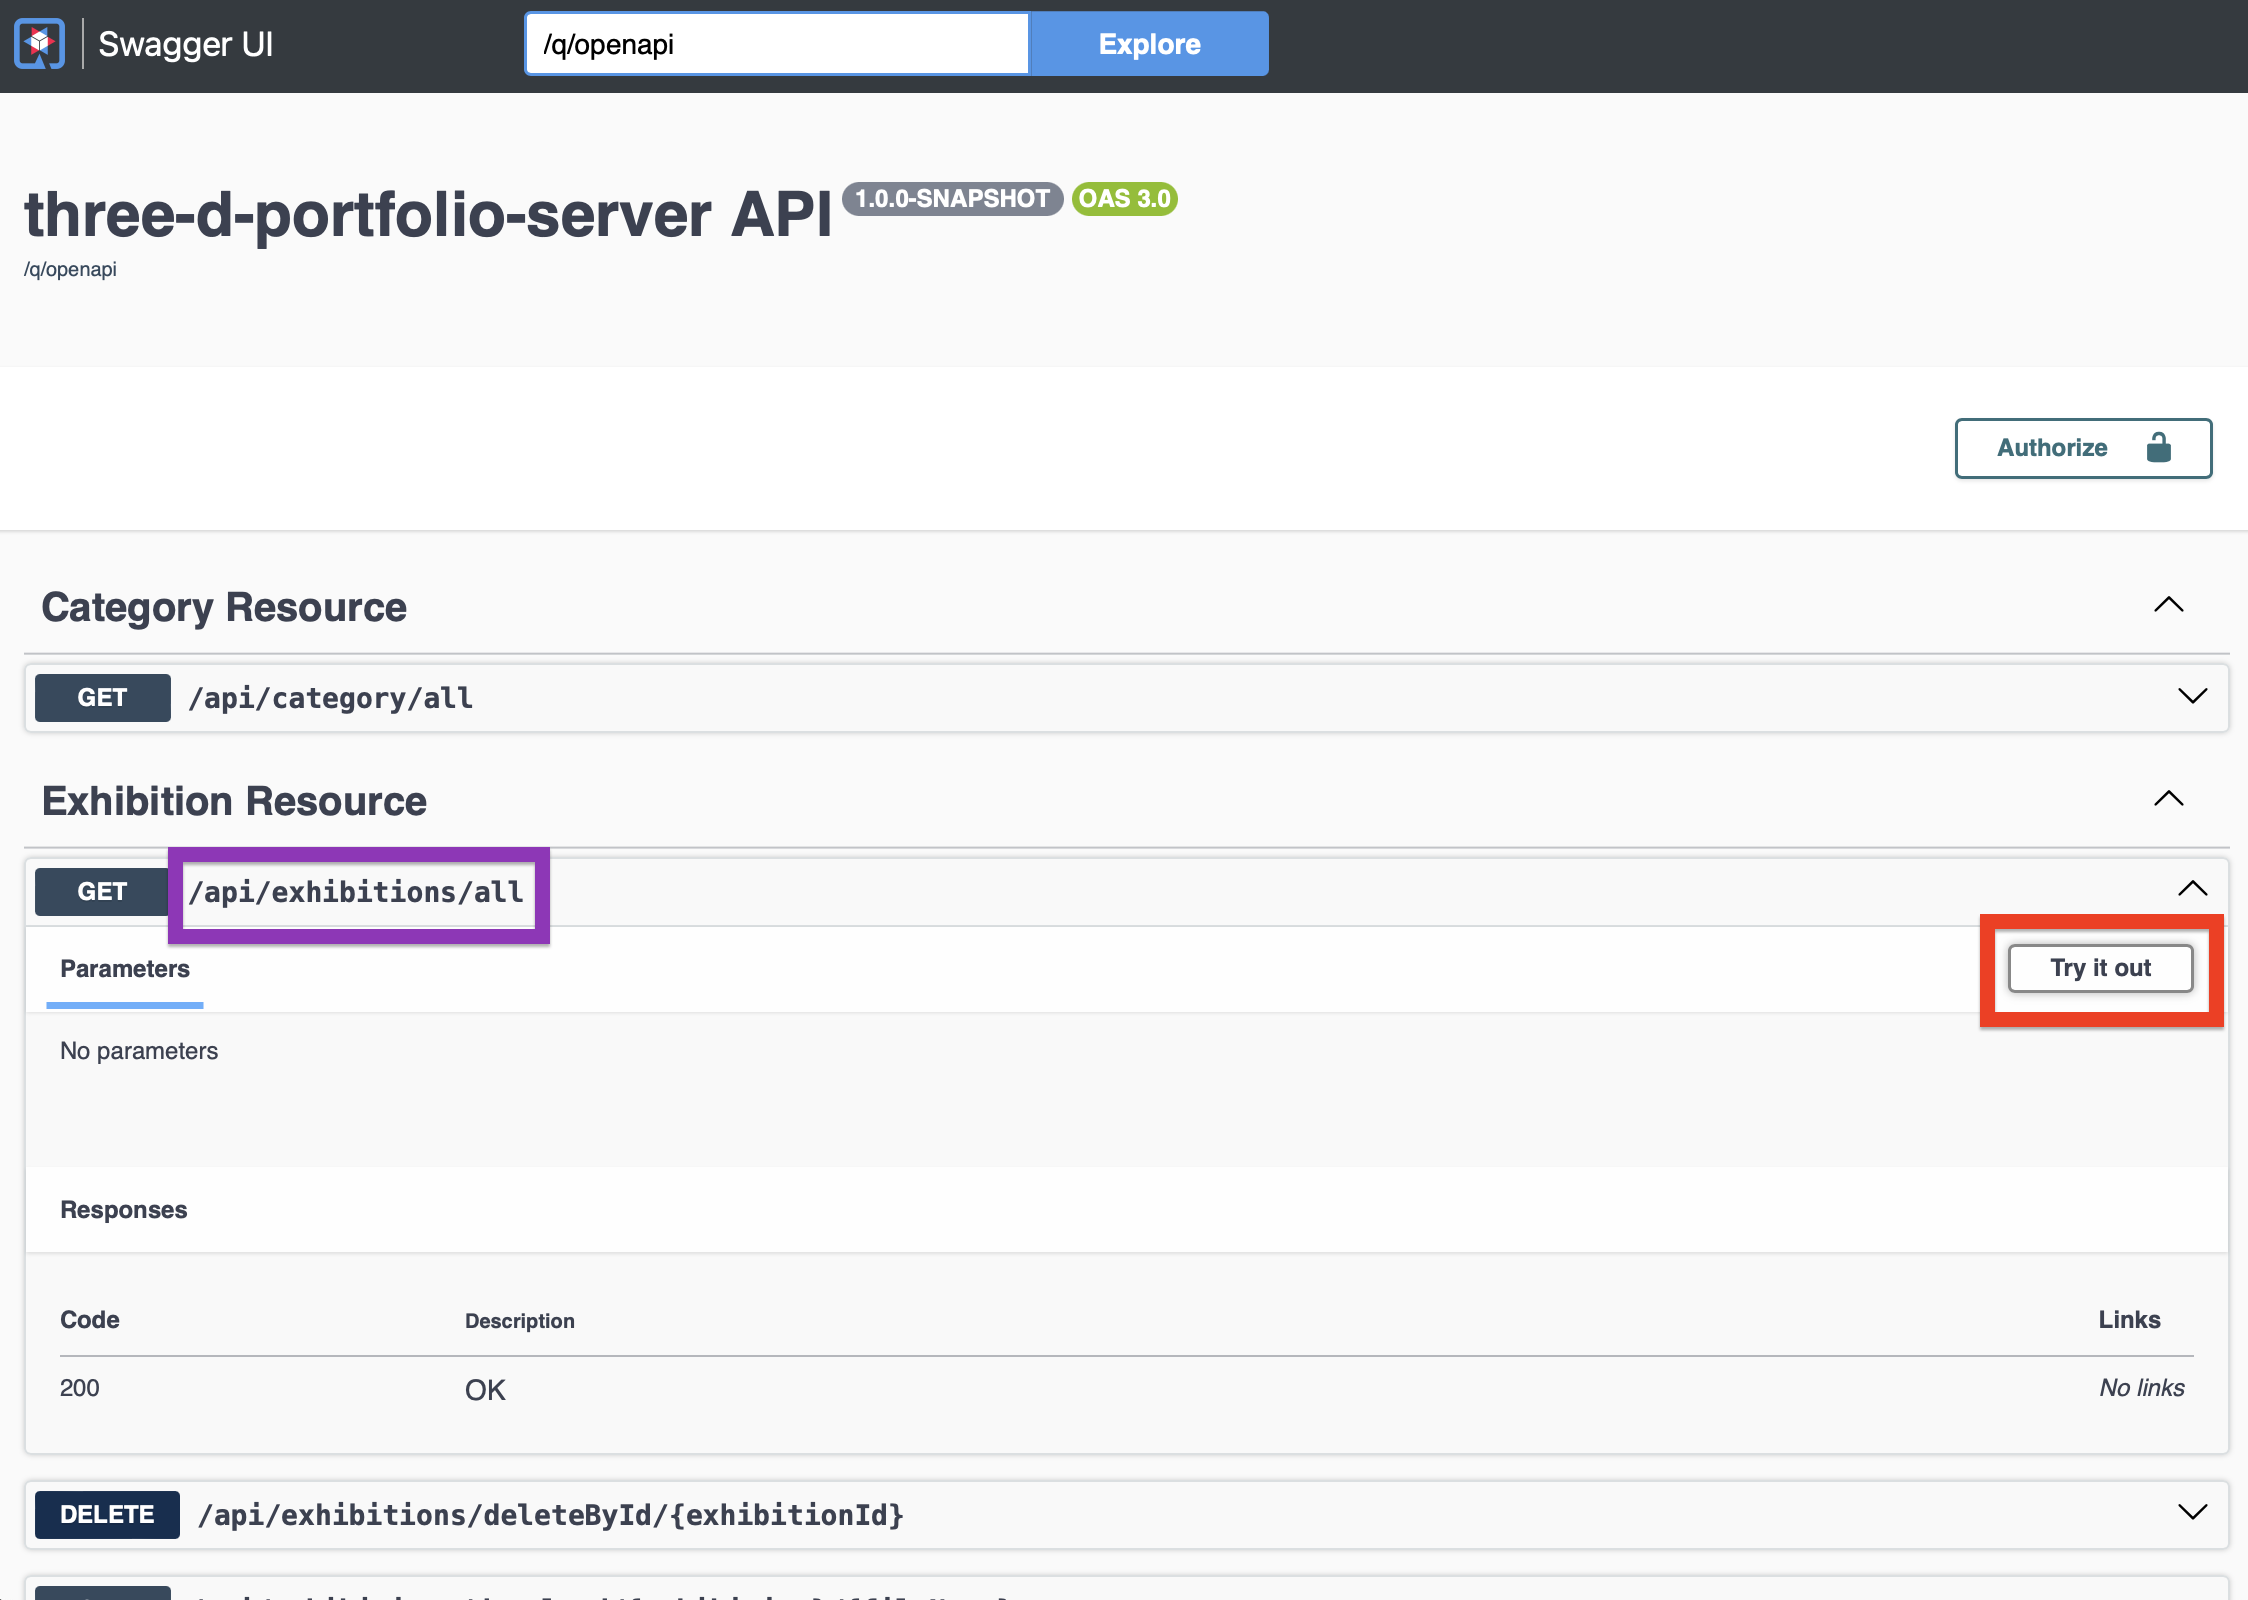
\includegraphics[scale=0.3]{pics/swaggerui.png}
    \caption{Übersicht der erstellten Schnittstellen}
    \label{fig:implementation:swaggerui}
\end{figure}

In Abbildung \ref{fig:implementation:swaggeruipost} lässt sich erkennen, dass die generierte Abfrage für numerische Werte standardmäßig \emph{0} und alphabetische Sequenzen \emph{string} einsetzt. 
Zweiteres ist kein Problem, da jedoch beim Anlegen jedes neuen Objekts die Id generiert wird, ist es einfacher, die Id aus dem Request zu entfernen. 
Falls jedoch ein bestimmter Wert für dieses Attribut gewünscht ist, muss die Einzigartigkeit der angelegten Entitäten beachtet werden. 
Ansonsten werden neue Objekt womöglich nicht gespeichert.

\begin{figure}
    \centering
    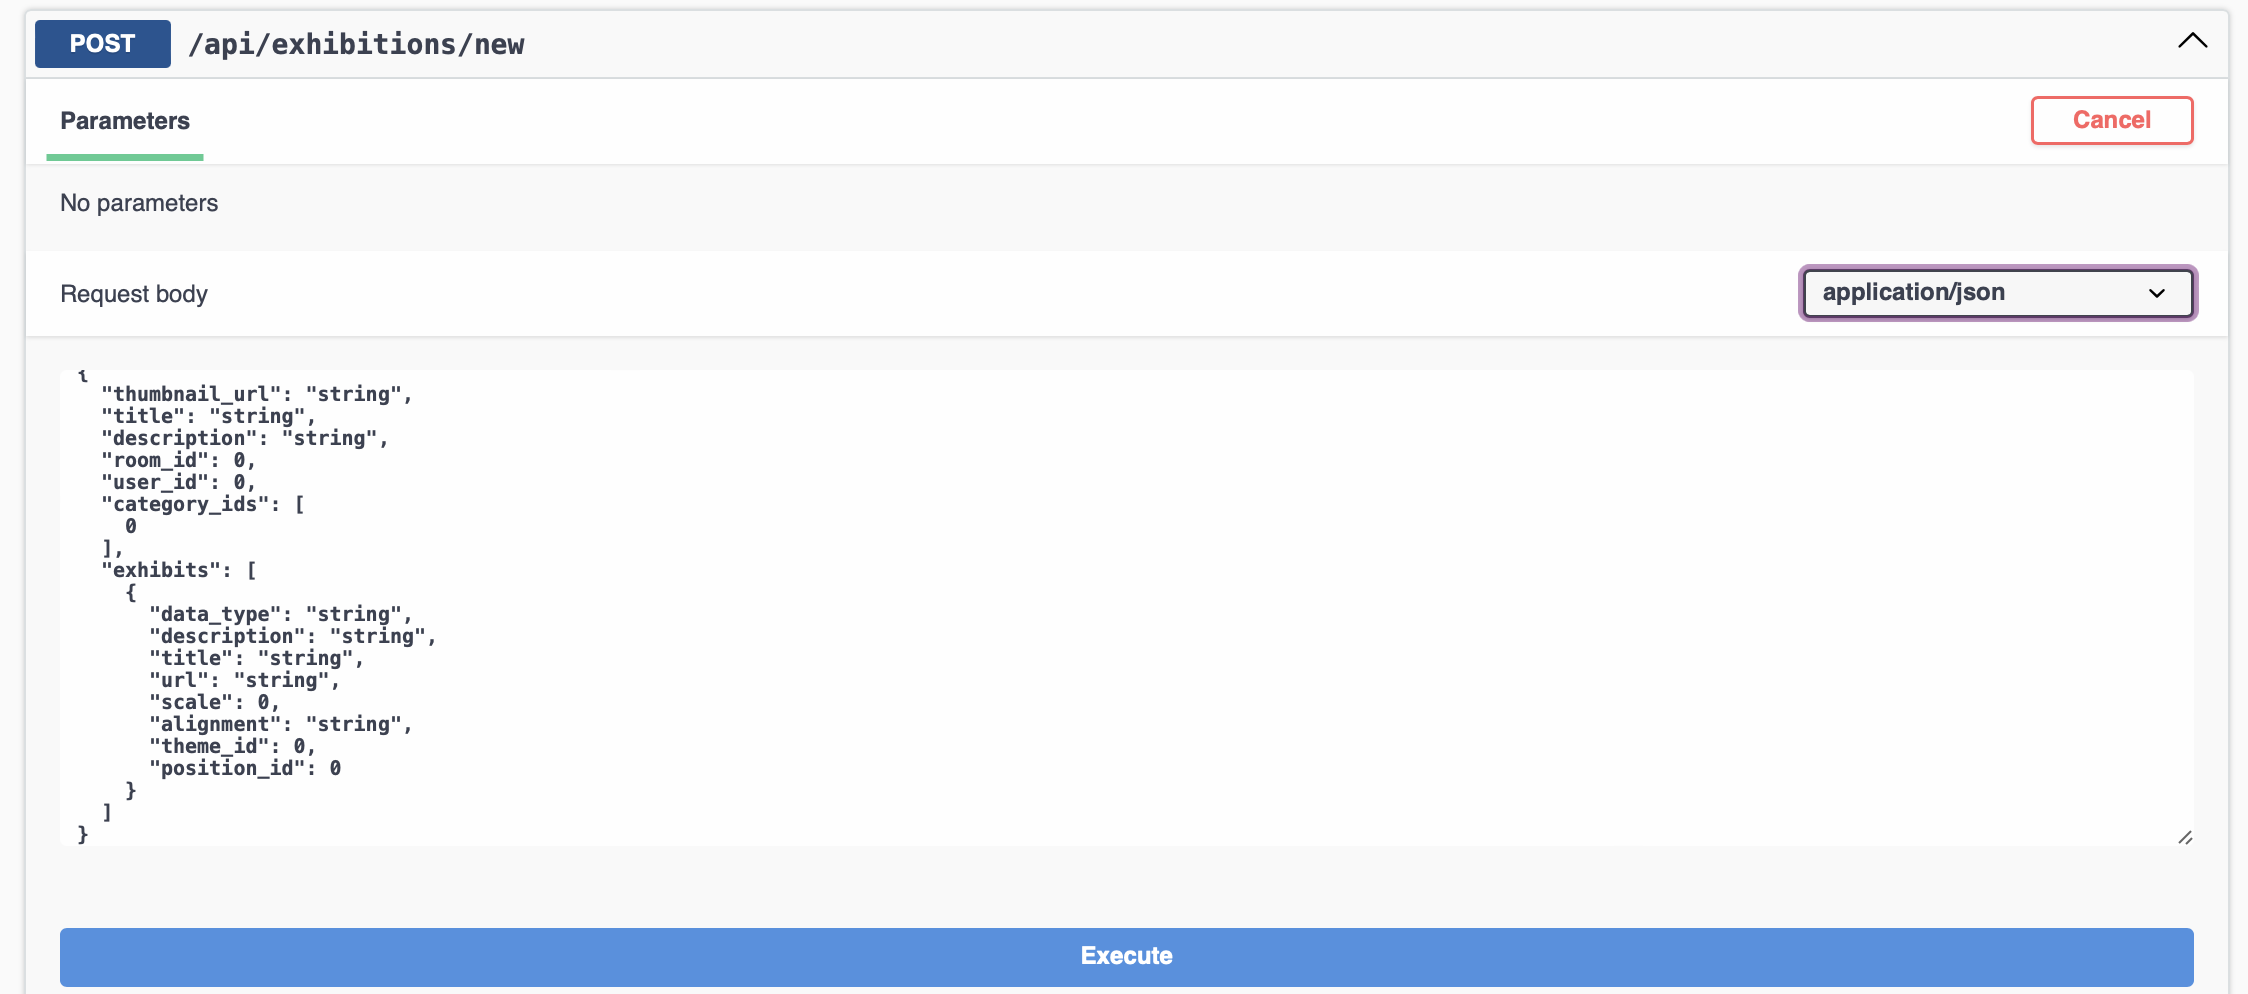
\includegraphics[scale=0.3]{pics/swaggeruipost.png}
    \caption{Automatisch generierte JSON-Anfrage}
    \label{fig:implementation:swaggeruipost}
\end{figure}

\subsection{Nach der Entwicklung}

In dieser Arbeit wird mit JUnit 5 und Mockito gearbeitet. 
Mockito ermöglicht es, die Repositories zu rekonstruieren. 
Diese Rekonstruktion werden \emph{Mocks} genannt.
\cite{quarkusMockAbout}
\begin{lstlisting}[label=JUnit 5 Abhängigkeit in pom.xml, language=xml]
<dependency>
    <groupId>io.quarkus</groupId>
    <artifactId>quarkus-junit5-mockito</artifactId>
    <scope>test</scope>
</dependency>
\end{lstlisting}

Tests in Quarkus werden mit \emph{@QuarkusTest} gekennzeichnet. 
Mocks werden durch \emph{@InjectMock} erstellt.
Diese stellen alle Methoden aus den gemockten Repositories zur Verfügung.
Zusätzlich besteht die Möglichkeit zu definieren, dass eine Methode vor jedem Test ausgeführt werden soll mittels \emph{@BeforeEach}. 
Die einzelnen Tests werden zusätzlich mit \emph{@Test} annotiert. 
\cite{quarkusMockAbout}

Durch die Priorisierung des Testvorganges während der Entwicklung, wurden die zusätzlich angelegten Testklassen nur für die wichtigsten Endpoints genutzt. 
Dazu zählt beispielsweise die Entität Exhibition. 
Im unteren Beispiel wird ein Requst auf den Endpoint \emph{api/exhibits/} erstellt, wobei keine Exhibition vorhanden ist. 
Dadurch wird der Statuscode 404 erwartet. 
\begin{lstlisting}[label=Ein Exhibition Test, language=Java]
@Test
public void testGetExhibitByIncorrectId() {
    given()
            .when()
            .pathParam("exhibitionId", 1L)
            .get("/api/exhibitions/{exhibitionId}")
            .then()
            .statusCode(404);
}
\end{lstlisting}
